\section{Basic Methods}
\label{BasicM}
In order to get some basic understanding of the methods commonly used for iris classification the work presented in an article is implemented. The work implemented is the work of \cite{Khan2017a} described in \citep{Khan2017a}.\todo{make sure references read right} In the work \gls{vl} images of the iris obtained by smartphones are processed and used to train different classifiers. The processing consists of a sequence of steps. The steps included are

\begin{itemize}
\item Iris Detection
\item Eyelid Suppression
\item Iris Normalisation
\item Noise Removal
\item Histogram Equalisation 
\item Feature Extraction
\item Training and Classification
\end{itemize}
\autoref{fig:ExWars} shows an example of an image from the database. Before the first step some simple preprocessing was done. The red channel is preserved and the other two other colour channels are neglected. This is done because this simulates the use of \gls{nir} light. The result is a greyscale image based on the red channel. In the following sections the implementation of each of the steps will be elaborated. 

\begin{figure}[h]
\centering
\begin{subfigure}{.47\textwidth}
\centering
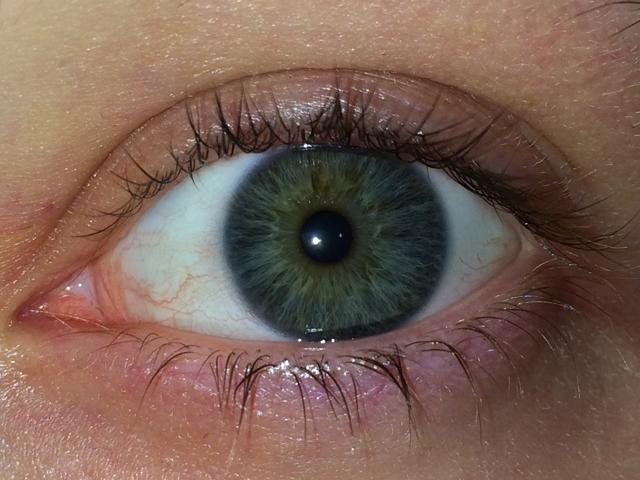
\includegraphics[width=0.90\textwidth]{IMG_1838.jpg}
\caption{Example of visible light image of an iris from the used database.}
\label{fig:ExWars}
\end{subfigure}
~
\begin{subfigure}{.47\textwidth}
\centering
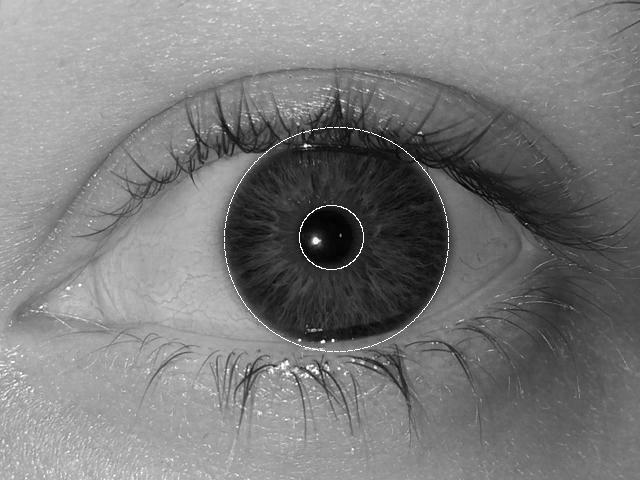
\includegraphics[width=0.90\textwidth]{0002left_13-marked.jpg}
\caption{The eye marked with the identified edges of the iris.}
\label{fig:MarkedI}
\end{subfigure}
\end{figure}



\subsection{Iris Detection}
The first step of processing is locating the iris. For this purpose Daugman's Integro-differential operator was used. The operator identifies the circular contour, which has the greatest change in intensity by varying the three parameters defining the circle. \autoref{fig:MarkedI} shows an example of the identified edges of the iris.



\subsection{Eyelid Suppression}

\subsection{Iris Normalisation}
For the normalisation Daugman's rubber sheet model is used. The purpose is to get a rectangular image of the iris, which corresponds to taking the annulus covered by the iris region, cutting it open and unfolding or stretching it to a rectangular shape. 

The model does this by mapping from polar coordinates based on radius and angle in the annulus to a rectangle where the angle is on the x-axis and the radius is on the y-axis of the image. 
This was implemented using a function in the library crated my Libor Masek.




\begin{figure}[h]
\centering
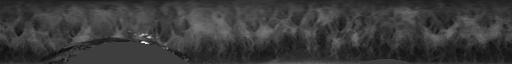
\includegraphics[width=\textwidth]{002polar.jpg}
\caption{The normalised image of the iris before applying functions.}
\label{fig:SimPolar}
\end{figure}

\subsection{Noise Removal}
Though the article uses several well known methods which are commonly used in processing of images of irises, their descriptions of the methods are quite inadequate. After obtaining the normalised iris, the next step applied is noise removal. The purpose of the noise remover function is to remove noise occurring in the form of eyelashes covering parts of the iris. Usually the pixels showing the lashes will be among the darkest pixels. Since every image of the iris is different and how dark the iris is also varies, a threshold has to be identified adaptively. The article does not describe in depth how this is implemented, it simply states that some histogram analysis is done in order to obtain the lowest pixel values. \autoref{fig:histBif} shows the histogram of the normalised image before any noise removal. 

\begin{figure}[h]
	\centering
	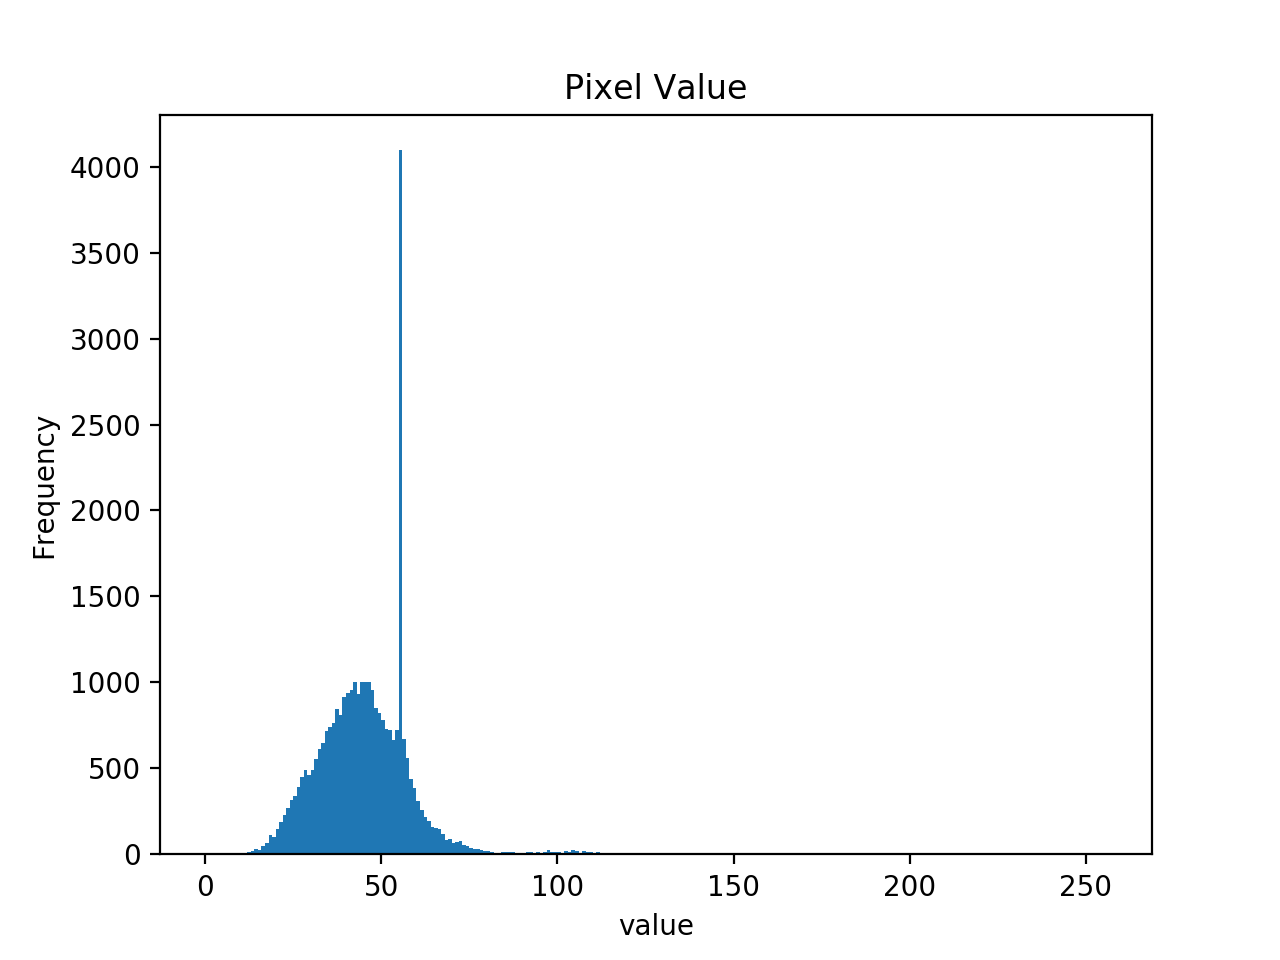
\includegraphics[width=0.7\textwidth]{hist_before.png}
	\caption{The histogram before applying the functions.}
	\label{fig:histBif}
\end{figure}

As the information about the exact approach used in the article is inadequate, an adaptive algorithm is created. The algorithm implemented identifies a threshold value based on the histogram. This is done by first identifying the highest and lowest bin-value, which has a frequency of more than a specified "recognition value", which was set to 10 in this project. The recognition value is introduced to make sure outliers are not defining for the threshold. Afterwards the threshold is calculated by the formula in \autoref{eq:pix_threshold}, where "Fraction" \todo[author=Niclas]{Skal vi evt lave variable fra ligninger skråskrift i stedet?} is a parameter set manually defining how large a part of the identified pixel value range has to me thresholded. During the processing in this project "Fraction" was set to be equal $0.1$. 

\begin{equation}\label{eq:pix_threshold}
	\text{Threshold}=\text{Low~Value}+\text{Fraction}\cdot(\text{High~Value}-\text{Low~Value})
\end{equation}


After the threshold has been found it is applied to all pixels in the image. The pixels lower than the threshold are eliminated and have to be reconstructed from neighbouring pixels. Also here the article provides very limited information about the algorithm applied. Therefore an algorithm was implemented, which restores pixels from non-occluded neighbour regions. A part of the algorithm identifies the pixels with values lower than the threshold and saves the pixel coordinates of the pixels. The saved pixels are  reconstructed iteratively from neighbouring pixels following the 4-connectivity principle. The pixels are reconstructed when there are at least 2 neighbour pixels they can be reconstructed from. They are only reconstructed from pixels above the threshold, this can be pixels that initially were above the threshold, or it can be pixels that have already been reconstructed. The pixels are reconstructed by assigning the average of the neighbours with values above the threshold as the new pixel value. Once all thresholded pixels have been reconstructed the reconstructed image is returned.

Because the eliminated pixels are reconstructed only from pixels with a value higher than the threshold there are certain traits that can be expected in the histogram of the reconstructed image. One of the traits is that there is a flatline from 0 to the threshold value. A second trait is that a peak close to the threshold is likely to occur because the eliminated values are reconstructed from neighbours which are likely to be close to the value of the eliminated pixels. However, the plotted histogram after reconstruction is as shown in \autoref{fig:histSpill}.

\begin{figure}[h]
	\centering
	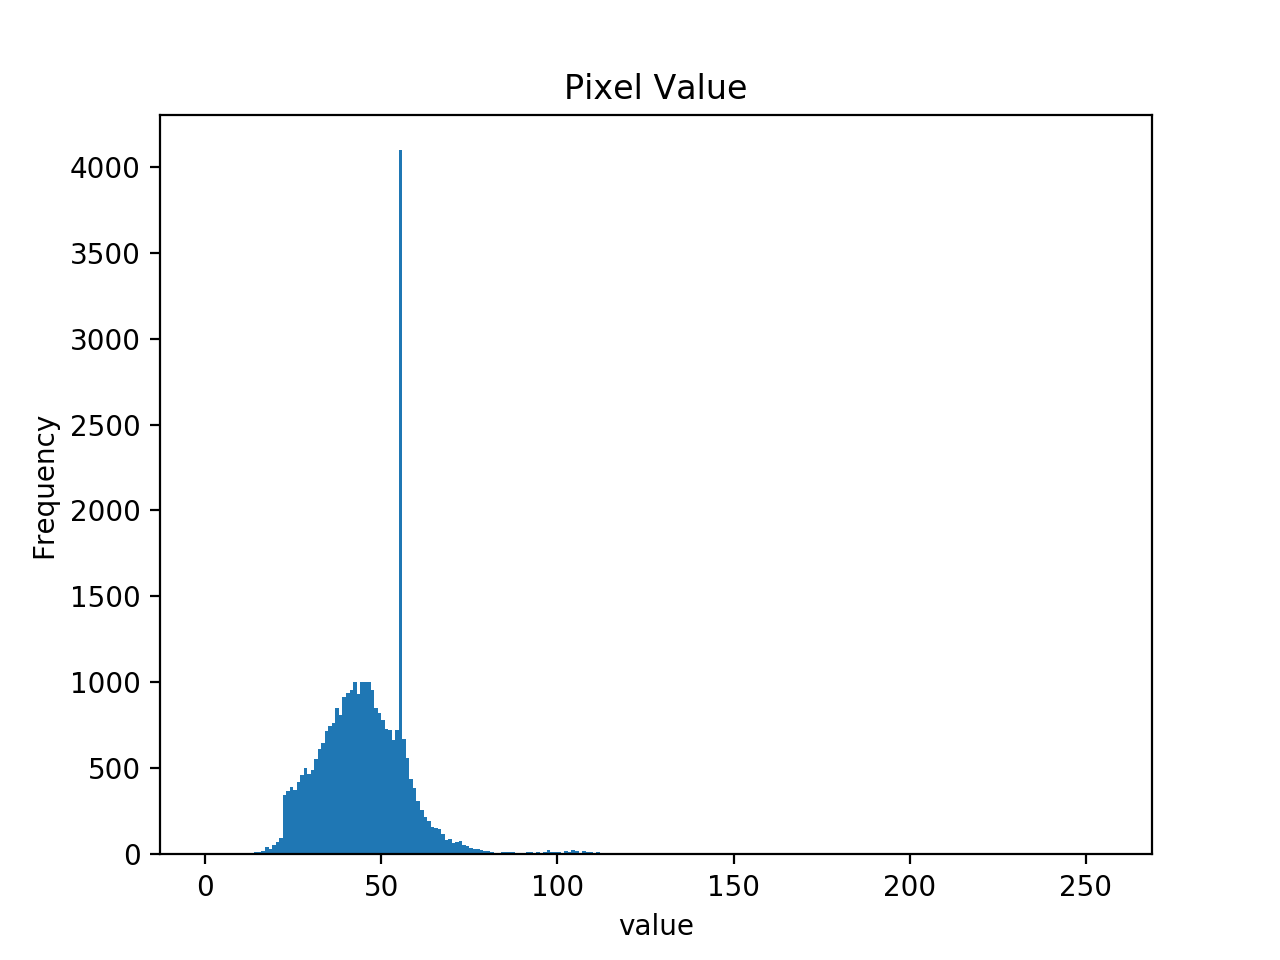
\includegraphics[width=0.7\textwidth]{hist_spill.png}
	\caption{The histogram of the image after reconstruction of pixels.}
	\label{fig:histSpill}
\end{figure}

As can be seen there is a small peak as expected, however, there seem to be a "spill over" across the threshold to the lower values. By closer examination of the code it was discovered that this was caused due to a programming mistake. The mistake was that the values used for reconstruction were obtained from the original image and not from the reconstructed image. Once this mistake was corrected the histogram was as expected as shown in \autoref{fig:histFine}. 

\begin{figure}[h]
	\centering
	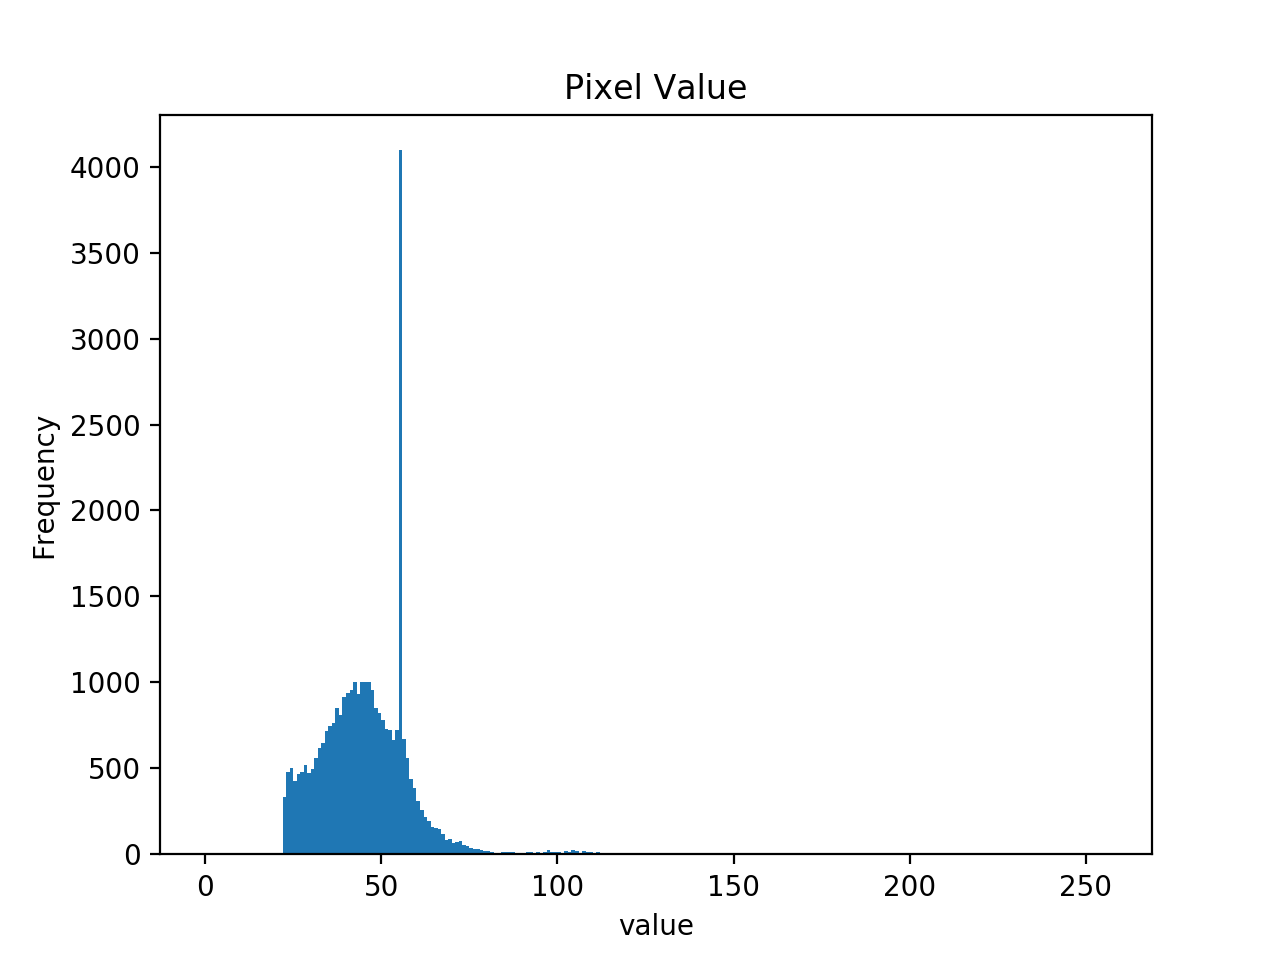
\includegraphics[width=0.7\textwidth]{hist_nicespacing.png}
	\caption{The histogram of the image after applying the corrected noise remover function.}
	\label{fig:histFine}
\end{figure}

In relation to the reconstruction of pixels it should be noted that it could have been done with 8-connectivity, and the iterative process could be split up to more steps, such that pixels are always constructed from as many neighbours as possible. This may give a better reconstruction, however, this has not been investigated. 
Furthermore, small tests showed that the adaptive threshold is difficult to define in an optimal way. If the threshold is too low the eyelash might be reconstructed from edge pixels of the eyelash creating just a lighter eyelash, which is still darker than the iris in the background. If the threshold is higher, it might eliminate the eyelashes, but also be destructive to darker parts of the iris. Maybe this could also be solved if the reconstruction happened based on the neighbourhood and not just the most adjacent neighbour pixels.
 
During implementation the histograms were frequently inspected in order to ensure the results were as expected. \autoref{fig:HistEli} shows a histogram with some eliminated pixel values. It turns out that the function used for generating histograms in python by default takes the range of the pixel values and splits that into as many bins as specified. As a result some of the bins cover a range of values that is entirely between two integer values and thus do not count any instances of pixel values as they are always integers between 0 and 225. This was solved by passing a specific range (0:256) as an argument and then the histogram was as described in \autoref{fig:histFine}.

\begin{figure}[h]
	\centering
	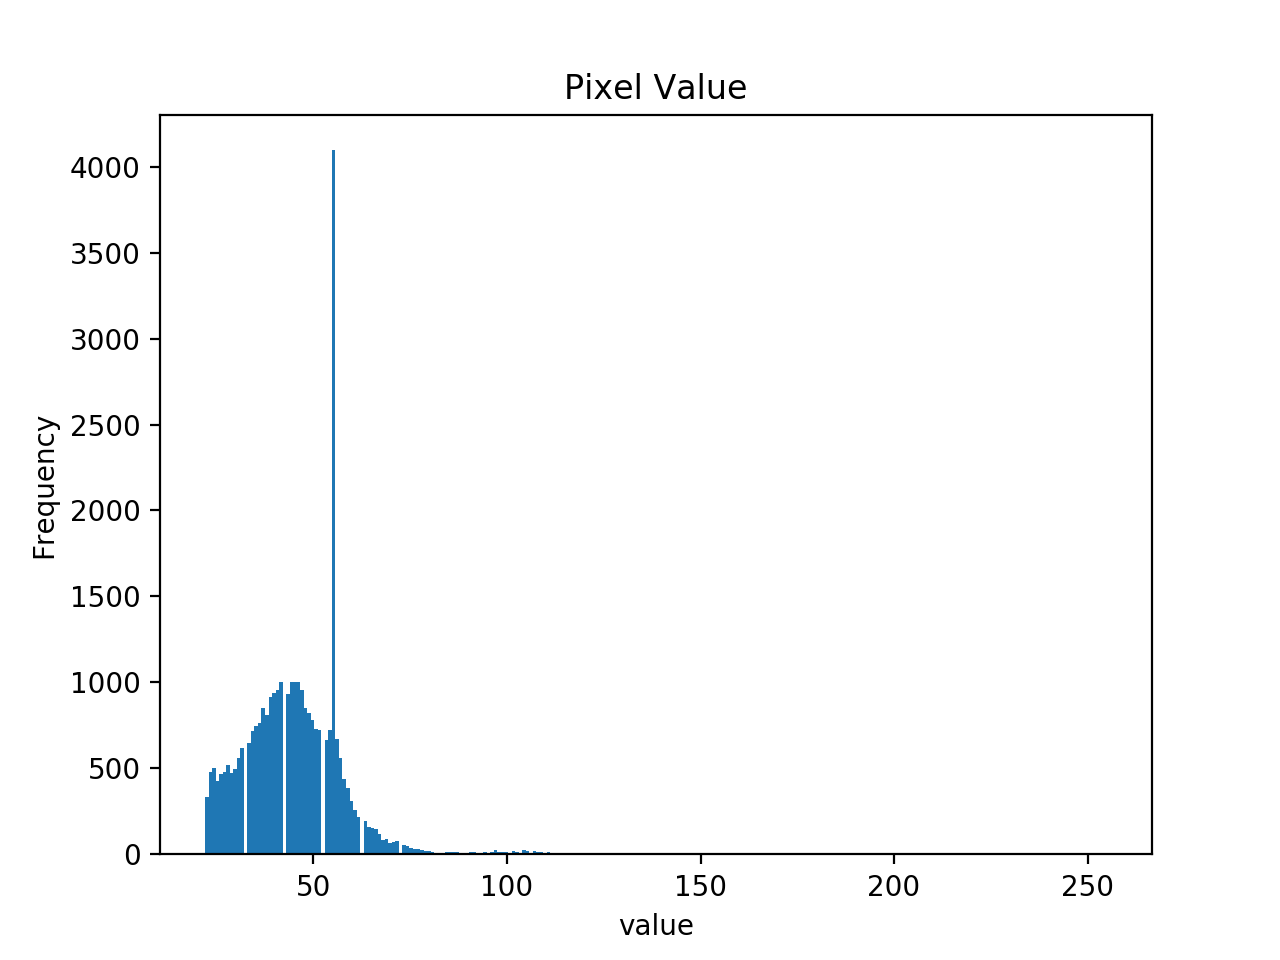
\includegraphics[width=0.7\textwidth]{hist_troublespacing.png}
	\caption{The histogram of the reconstructed image with eliminated values.}
	\label{fig:HistEli}
\end{figure} 

\subsection{Histogram Equalisation}
The histogram equalisation is applied to increase contrast. This is necessary to enhance the structures in the iris. This was implemented manually. Just as in the noise removal the lowest and highest bin values with more instances than a specified value are found. Based on the values found the histogram is stretched using the formula in \autoref{eq:hist_stretch}.

\begin{equation}\label{eq:hist_stretch}
	\text{New~Pixel~Value}=(\text{Pixel~Value}-\text{Low~Value})\cdot\frac{255}{\text{High~Value}-\text{Low~Value}}
\end{equation}

The pixels, which have values above $ 255 $ or below $ 0 $ after the formula is applied, are set to $ 255 $ or $ 0 $ respectively. The resulting image is shown in \autoref{fig:irisST}, while \autoref{fig:histST} shows the histogram after applying the formula to each pixel.
\begin{figure}[h]
\centering
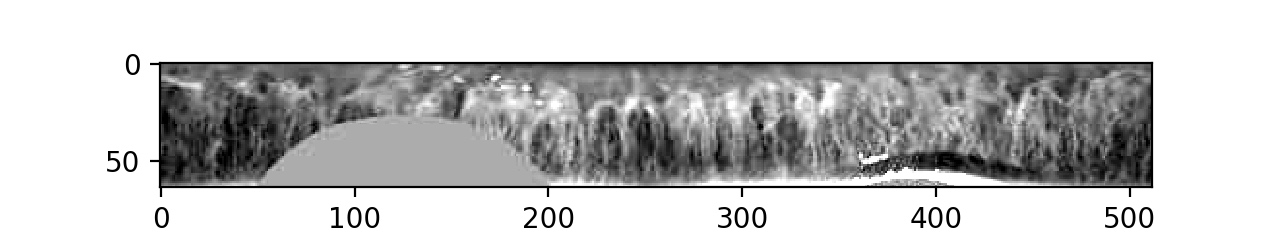
\includegraphics[width=\textwidth]{Stretch_iris.jpg}
\caption{The image of the iris after applying the initial "equalise histogram" function.}
\label{fig:irisST}
\end{figure}
\begin{figure}[h]
\centering
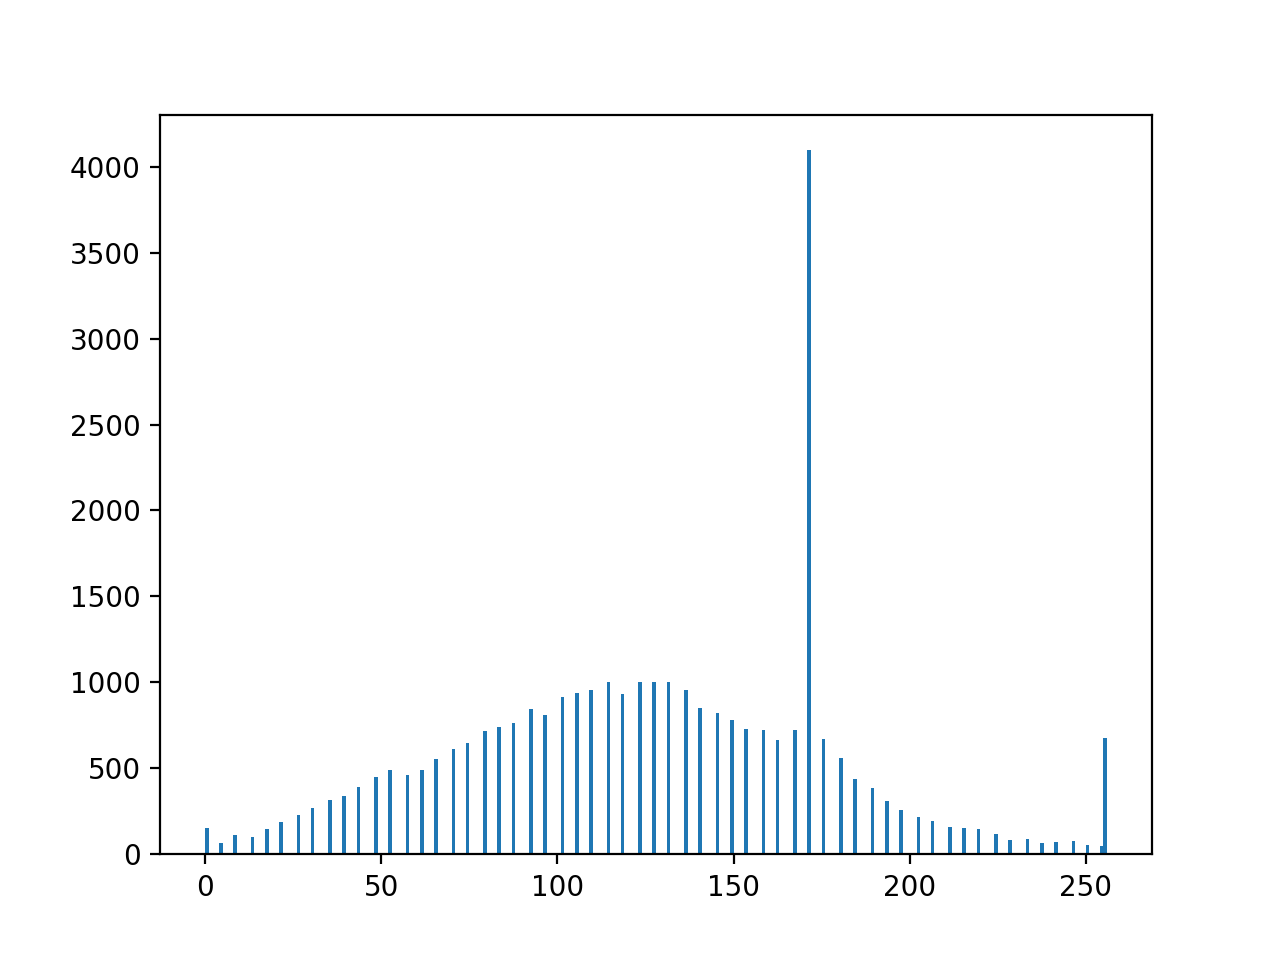
\includegraphics[width=0.7\textwidth]{Stretch_hist.png}
\caption{The histogram of the image after applying the initial "equalise histogram" function.}
\label{fig:histST}
\end{figure}
However, it was discovered that the implemented method was actually histogram stretching which was mistakenly taken as the same as histogram equalisation. Though the two methods have somewhat the same effects histogram equalisation is better at ensuring a uniform spreading of the pixels across the histogram. 
This is done by identifying a transform of the bin values which causes the \gls{cdf} of the histogram to be as linear as possible, and apply it to the grey levels or bin values. The result of the histogram equalisation is showed in \autoref{fig:irisEQ} and \autoref{fig:histEQ}.
\begin{figure}[h]
\centering
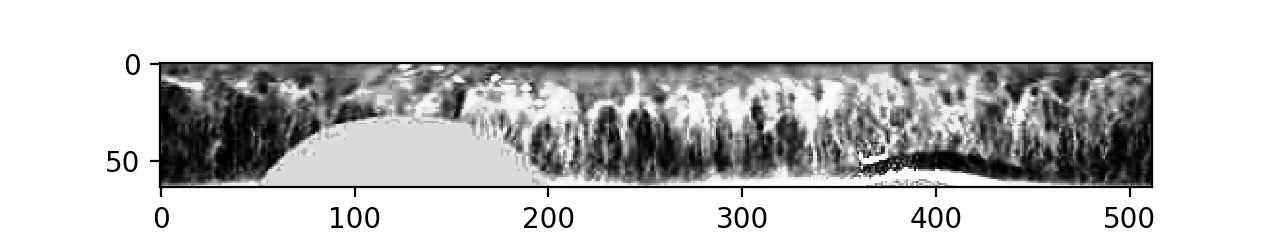
\includegraphics[width=\textwidth]{Equal_iris.jpg}
\caption{The image of the iris after applying the real equalisation of the histogram.}
\label{fig:irisEQ}
\end{figure}
\begin{figure}[h]
\centering
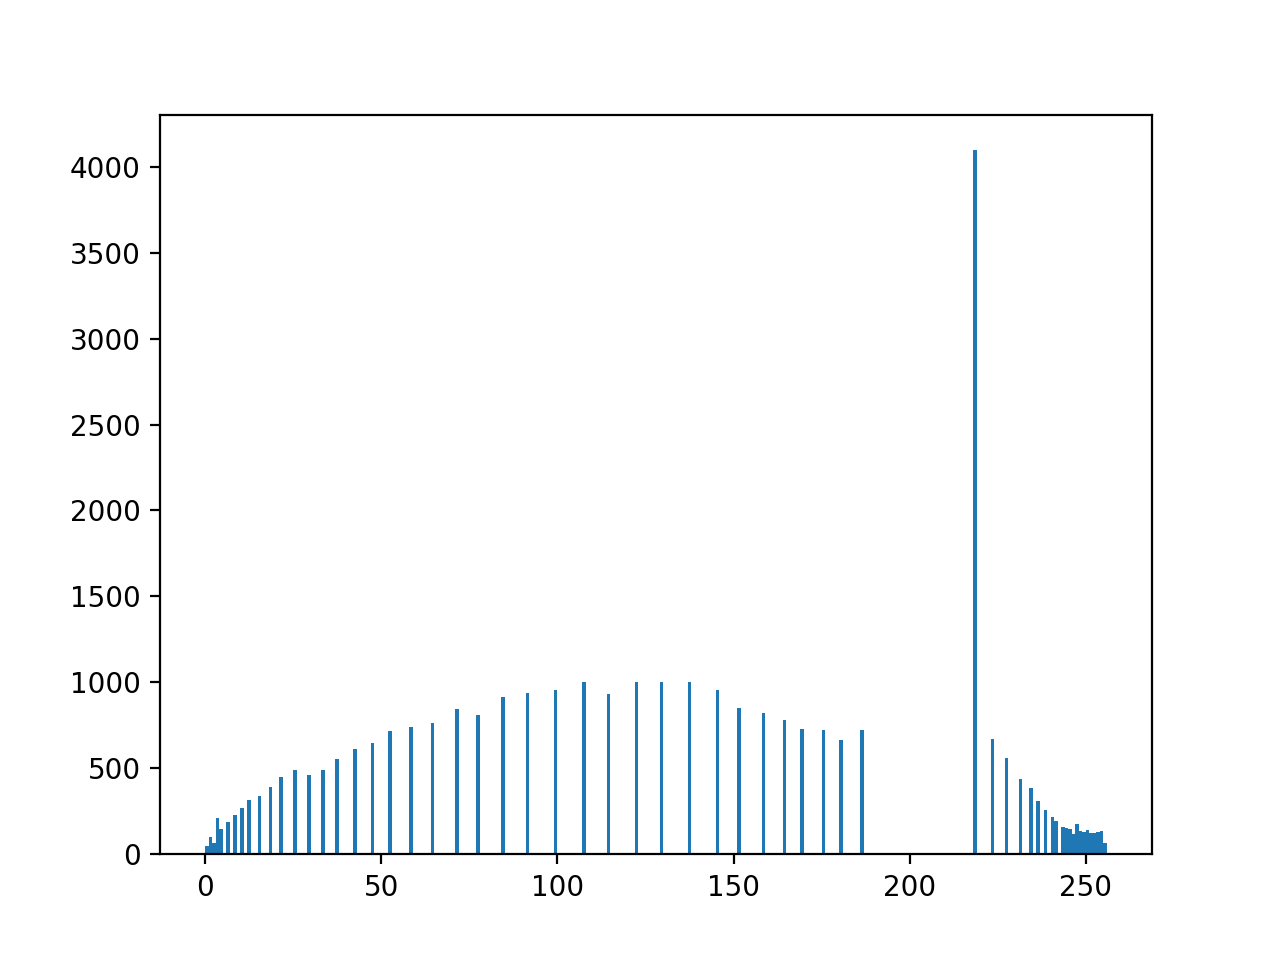
\includegraphics[width=0.7\textwidth]{Equal_hist.png}
\caption{The histogram of the image after applying the real equalisation of the histogram.}
\label{fig:histEQ}
\end{figure}
When comparing the two images of the iris after applying the two different contrast adjustment methods it can be concluded that the histogram equalisation does indeed result in better contrast and a more enhanced and out spoken appearance of the structures in the iris than the histogram stretching does. Testing also showed that using the equalisation rather than the stretching increased the accuracy, this is further addressed in \autoref{MachineLearnClassification}. 

\subsection{Feature extraction}
As it is difficult to extract all the complex structures in the iris the work presented uses the iris image as input. However, because the image in full will result in too large amounts of data to handle during feature extraction is done. Feature vectors are extracted using Haar wavelets in a wavelet decomposition. \todo[author=Niclas]{Der mangler noget i det afsnit her.}

Haar wavelets are a fast and simple way to obtain wavelets. In Haar wavelets the decomposition is done by calculating the average of neighbouring pixels as well as half the difference between neighbouring pixels. Due to the way the method works the image is lowpass or hi-pass filtered two times in each of the possible combinations. The image of the greatest interest in this case is the one that has been lowpass filtered in both horizontal and vertical direction, this is referred to at LL. This image will be a compressed version of the original image, showing an approximation or the tendency of the original image. The other images created in one stage are HH, HL, LH all of which contain detail coefficients. HH is representing the diagonal detail, while HL presents horizontal detail and LH presents vertical detail. The LL will naturally appear in the upper left corner of the output matrix. 

In order to compress the image sufficiently three stages or passes of Haar wavelet decomposition was carried out. The result is showed \autoref{fig:haar3}. 
\begin{figure}[h]
\centering
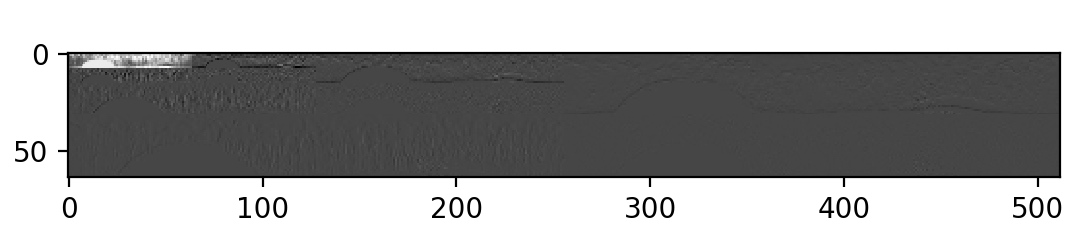
\includegraphics[width=\textwidth]{haar_3.jpg}
\caption{The result of the three level haar wavelet decomposition. Note that the small light image in the upper left corner is the LL3, which is used onwards.}
\label{fig:haar3}
\end{figure}
The resulting matrix of LL3 coefficients is then put into a feature vector, which is used for training the classifiers described in \autoref{MachineLearnClassification}.

\subsection{Training and Classification}
\label{MachineLearnClassification}
For classification different classifiers were tested. The investigated classifiers are the \gls{knn}, \gls{lda}, as well as a \gls{svm} with linear or quadratic kernel. In the section the theory behind the different classifiers will

\subsubsection*{K-Nearest Neighbour}
 \gls{knn} is one of the most simple supervised classification methods. It is a non-parametric method. This means that the train data is used "raw" and there are no parameters that are deducted from the data in order to form a model. 
 
 The way \gls{knn} 
\subsubsection*{Linear Discriminant Analysis}
\subsubsection*{Support Vector Mashines}

\subsubsection*{Cross Validation}












